% Two-page succession feature for Den Rullende Sten.
% Solid dark-red lines are direct named descent. The solid blue connector is a
% documented collateral line, abbreviated here to fit the newspaper page.

\definecolor{ImperialRed}{HTML}{711A22}
\definecolor{ImperialDarkRed}{HTML}{3A1116}
\definecolor{ImperialGold}{HTML}{BF8B2E}
\definecolor{ImperialCream}{HTML}{F5EEDC}
\definecolor{ImperialInk}{HTML}{24191A}
\definecolor{RebelRed}{HTML}{9B2F25}
\definecolor{ChurchGold}{HTML}{B68A26}
\definecolor{WinterBlue}{HTML}{294B6D}

\newcommand{\PortraitCrop}[3]{%
  \includegraphics[
    width=#1,
    height=#2,
    keepaspectratio,
    trim=45 250 45 0,
    clip
  ]{#3}%
}

% Keep portrait and faction mark optically centred on a shared midline.
% #1/#2 = portrait box, #3 = portrait file, #4 = mark, #5 = gap.
\newcommand{\PortraitLockup}[5]{%
  \makebox[\linewidth][c]{%
    \begin{tabular}{@{}c@{\hspace{#5}}c@{}}
      \raisebox{-0.5\height}{\PortraitCrop{#1}{#2}{#3}} &
      \raisebox{-0.5\height}{#4}
    \end{tabular}%
  }%
}

\newcommand{\ImperialMark}{%
  
\includegraphics[width=13mm]{assets/royal/Imperiet.jpg}%
}

\newcommand{\TaliaMark}{%
  
\includegraphics[width=13mm]{assets/royal/Talia-rebel-crown.png}%
}

\newcommand{\SeverinMark}{%
  
\includegraphics[width=13mm]{assets/royal/Severin-church-crown.png}%
}

\newcommand{\IsmareldaMark}{%
  
\includegraphics[width=13mm]{assets/royal/Ismarelda-winter-crown.png}%
}

\tikzset{
  family card/.style={
    draw=ImperialGold,
    line width=0.7pt,
    fill=white,
    rounded corners=1.2mm,
    inner sep=1.5mm,
    align=center
  },
  claim card/.style={
    draw=ImperialGold,
    line width=0.75pt,
    fill=white,
    rounded corners=1.2mm,
    inner sep=1.8mm,
    align=left
  },
  family line/.style={
    draw=ImperialDarkRed,
    line width=0.85pt
  },
  archive branch/.style={
    draw=WinterBlue,
    line width=1.05pt
  }
}

% ============================================================
% PAGE ONE - THE NEW SUCCESSION TREE
% ============================================================

% Always begin this feature on an even-numbered logical newspaper page.
\clearpage
\ifodd\value{page}
  % If a parity page is needed, use it to thank the academy's patron.
  \thispagestyle{empty}
  \vspace*{-\topskip}
  \noindent
  \begin{tikzpicture}[x=1mm,y=1mm,baseline=(thankbase)]
    \path[use as bounding box] (0,0) rectangle (116,-178);
    \coordinate (thankbase) at (0,0);

    \draw[ImperialDarkRed,line width=1.2pt] (-18,10) rectangle (118,-188);
    \draw[ImperialGold,line width=0.45pt] (-16,8) rectangle (116,-186);

    \node[anchor=north west,align=left,text width=110mm]
      at (1,-1) {%
        {\sffamily\bfseries\scriptsize\color{ImperialRed}
         DET GLEMTE AKADEMI TAKKER}\par
        \vspace{0.4mm}
        {\sffamily\bfseries\fontsize{17}{18}\selectfont
         KONG DORIAN VINTERKRONE}\par
        \vspace{0.5mm}
        {\sffamily\small\itshape\color{black!66}
         Konge af A'kastin}%
      };

    \fill[ImperialDarkRed] (1,-25) rectangle (113,-28);

    \node[anchor=center] at (30,-91) {%
      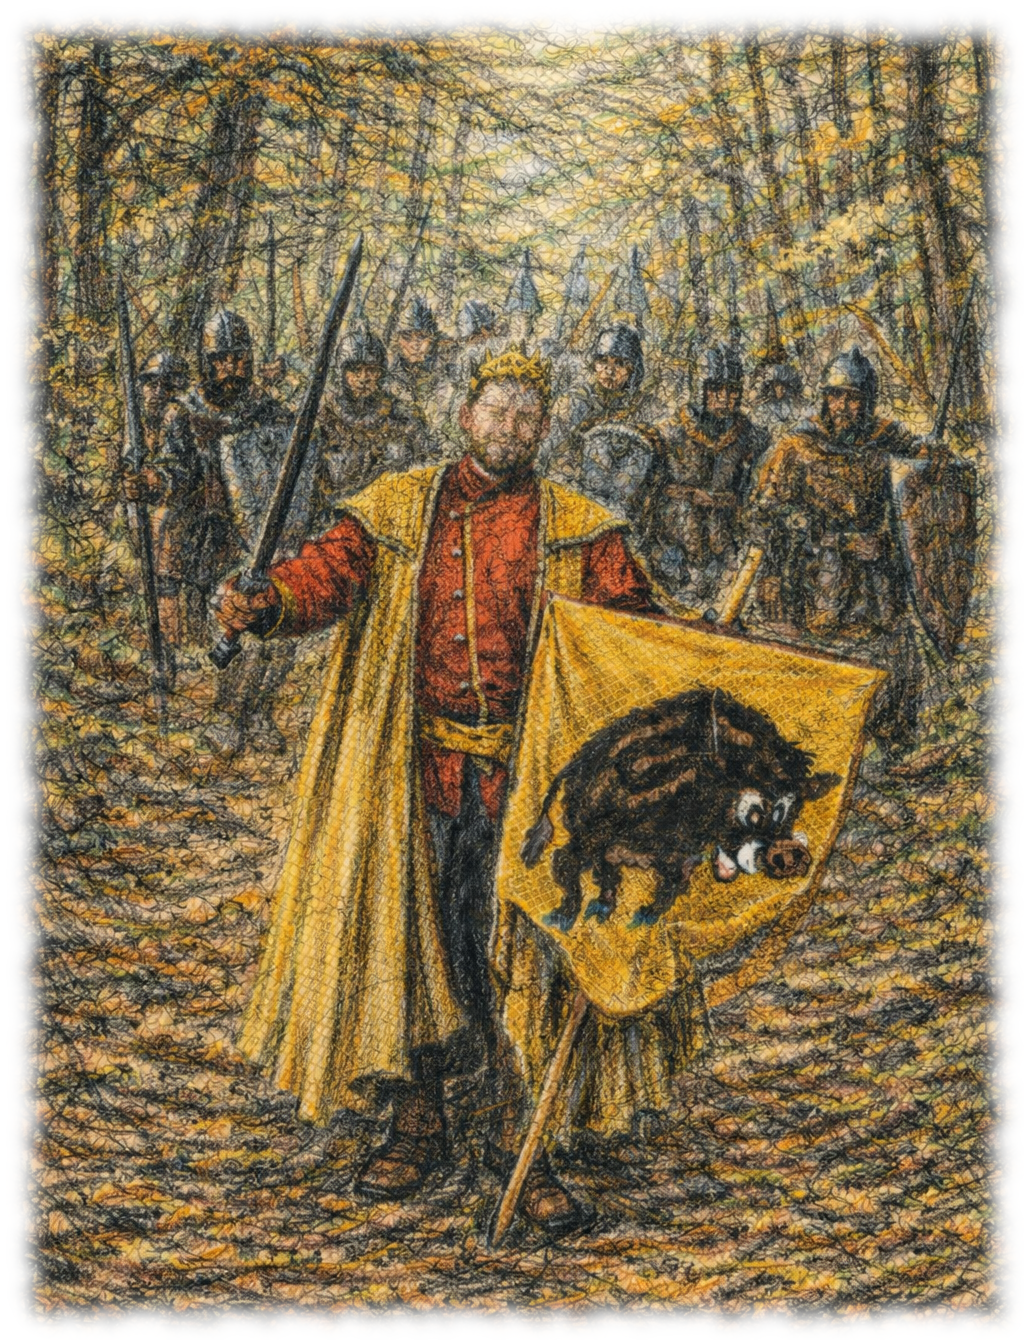
\includegraphics[height=103mm]{assets/royal/Kong Dorian.png}%
    };

    \node[
      anchor=north west,
      text width=40mm,
      align=center,
      fill=white,
      draw=ImperialGold,
      line width=0.8pt,
      rounded corners=1.2mm,
      inner sep=2.4mm
    ] at (69,-38) {%
      
\includegraphics[height=45mm]{assets/royal/vinterkroneSkjold.png}\par
      \vspace{1.4mm}
      {\sffamily\bfseries\scriptsize\color{WinterBlue}
       FOR STØTTEN TIL AKADEMIET}\par
      \vspace{1.2mm}
      {\sffamily\fontsize{7.2}{8.4}\selectfont\color{ImperialInk}
       Det Glemte Akademi takker Kong Dorian Vinterkrone for hans støtte til vores arbejde.\par
       \vspace{1.1mm}
       Hans hjælp holder blæk i husene, papir i trykpressen og budbringere
       på vejene, så nyheder og velunderbyggede rygter fortsat kan nå
      borgerene af Kalish.}\par
      \vspace{1.5mm}
      {\color{ImperialGold}\rule{29mm}{0.45pt}}\par
      \vspace{0.8mm}
      {\sffamily\bfseries\fontsize{6.7}{7.4}\selectfont
       MED TAKNEMMELIGHED\par
       REDAKTIONEN PÅ DEN RULLENDE STEN}%
    };

    \node[
      anchor=south west,
      align=center,
      text width=107mm,
      fill=ImperialDarkRed,
      text=white,
      inner sep=2.3mm
    ] at (1,-176) {%
      {\sffamily\bfseries\scriptsize
       Vi er stolte af at kunne sige at vi får støtte fra en sand helt blandt kujoner.}\par
      \vspace{0.5mm}
      {\sffamily\fontsize{6.8}{7.8}\selectfont
       Redaktionen håber at Kong Dorian får et langt og lykkeligt liv!}%
    };
  \end{tikzpicture}\par
  \clearpage
\fi
\thispagestyle{empty}
\vspace*{-\topskip}
\noindent

\begin{tikzpicture}[x=1mm,y=1mm,baseline=(pagebaseone)]
  \path[use as bounding box] (0,0) rectangle (116,-178);
  \coordinate (pagebaseone) at (0,0);

  \draw[ImperialDarkRed,line width=1.2pt] (-18,10) rectangle (118,-188);
  \draw[ImperialGold,line width=0.45pt] (-16,8) rectangle (116,-186);
  \coordinate (NW) at (0,0);

  \node[anchor=north west,align=left,text width=105mm]
    at ([xshift=1mm,yshift=-1mm]NW) {%
      {\sffamily\bfseries\scriptsize\color{ImperialRed}
       EKSTRA: SLAGET OM ARVEFØLGEN}\par
      \vspace{0.3mm}
      {\sffamily\bfseries\fontsize{18}{19}\selectfont
       DEN RØDE TRONE STÅR TOM}\par
      \vspace{0.5mm}
      {\sffamily\small\itshape\color{black!70}
       Aurelia er død.\\ Conrad er vendt tilbage.\\ Tre andre
       tronkrav nægter at bøje sig for ham.}%
    };



  \node[
    anchor=north west,
    text width=111mm,
    align=center,
    fill=ImperialDarkRed,
    text=white,
    inner xsep=1mm,
    inner ysep=1.1mm
  ] at ([xshift=1mm,yshift=-25mm]NW) {%
    \sffamily\bfseries\fontsize{6.6}{7.3}\selectfont
  };

  \node[
    family card,
    text width=29mm,
    minimum height=25mm
  ] (erik) at ([xshift=58mm,yshift=-46mm]NW) {%
    
\includegraphics[width=16mm,height=13mm,keepaspectratio]{assets/royal/Erik Fjendebane.png}\\[-0.7mm]
    {\sffamily\bfseries\scriptsize KEJSER ERIK II}\\[-0.3mm]
    {\sffamily\fontsize{6.2}{6.9}\selectfont\color{black!58}
     Faldt ved Sydporten}%
  };

  \coordinate (siblingsplit) at ([yshift=-5mm]erik.south);
  \draw[family line] (erik.south) -- (siblingsplit);
  \draw[family line] ([xshift=-30mm]siblingsplit) -- ([xshift=30mm]siblingsplit);

  \node[
    family card,
    text width=38mm,
    minimum height=38mm
  ] (conrad) at ([xshift=28mm,yshift=-85mm]NW) {%
    \PortraitLockup{22mm}{20mm}{assets/royal/Conrad Fjendebane.png}{\ImperialMark}{2mm}\\[1mm]
    {\sffamily\bfseries\small CONRAD FJENDEBANE}\\[-0.2mm]
    {\sffamily\fontsize{6.5}{7.3}\selectfont\color{black!62}
     Erik II's søn som marcherer mod Nordland\\
     \color{ImperialRed}\bfseries Levende eller Hrothgars gespenst?}%
  };

  \node[
    family card,
    draw=ImperialRed,
    line width=1.1pt,
    text width=38mm,
    minimum height=38mm
  ] (aurelia) at ([xshift=88mm,yshift=-85mm]NW) {%
    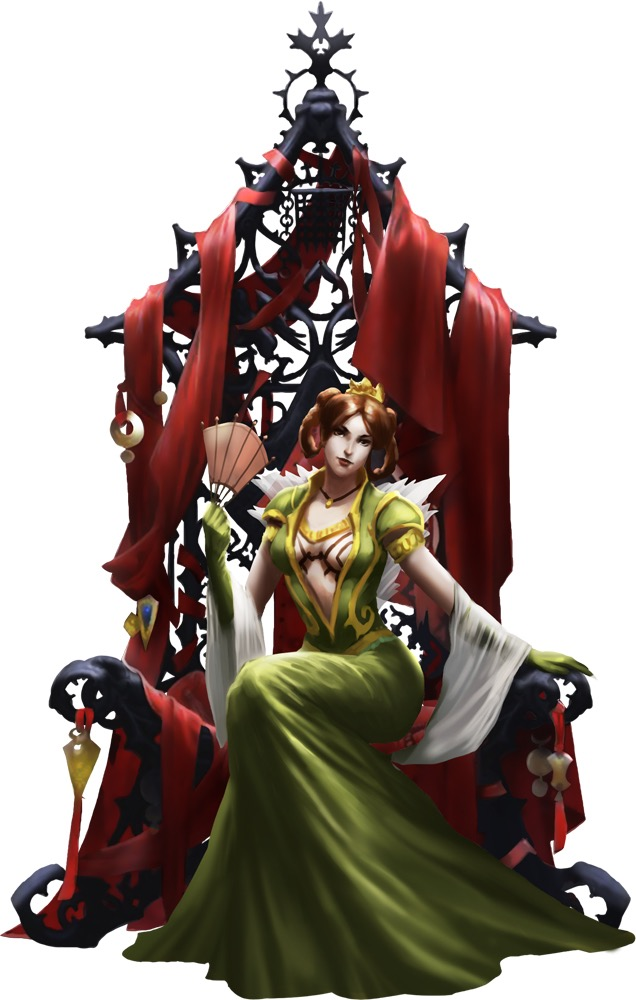
\includegraphics[width=27mm,height=23mm,keepaspectratio]{assets/royal/Aurelia Fjendebane.jpg}\\[-0.5mm]
    {\sffamily\bfseries\small KEJSERINDE AURELIA}\\[-0.2mm]
    {\sffamily\fontsize{6.7}{7.4}\selectfont\color{ImperialRed}\bfseries
     HVEM DRÆBTE KEJSERINDEN?}%
  };

  \draw[family line] ([xshift=-30mm]siblingsplit) |- (conrad.north);
  \draw[family line] ([xshift=30mm]siblingsplit) |- (aurelia.north);

  \coordinate (childsplit) at ([yshift=-5mm]conrad.south);
  \draw[family line] (conrad.south) -- (childsplit);
  \draw[family line] ([xshift=-14.5mm]childsplit) -- ([xshift=14.5mm]childsplit);

  \node[
    family card,
    draw=RebelRed,
    text width=30mm,
    minimum height=41mm
  ] (talia) at ([xshift=13.5mm,yshift=-132mm]NW) {%
    \PortraitLockup{16mm}{17mm}{assets/royal/Talia Fjendebane.png}{\TaliaMark}{1mm}\\[1mm]
    {\sffamily\bfseries\scriptsize TALIA FJENDEBANE}\\[-0.1mm]
    {\sffamily\fontsize{6.1}{6.8}\selectfont\color{black!62}
     Opvokset i Permersland\\
     \color{RebelRed}\bfseries Radikalt opgør mod blodretten}%
  };

  \node[
    family card,
    draw=ChurchGold,
    text width=30mm,
    minimum height=41mm
  ] (severin) at ([xshift=48.5mm,yshift=-132mm]NW) {%
    \PortraitLockup{16mm}{17mm}{assets/royal/Severin Fjendebane.png}{\SeverinMark}{1mm}\\[1mm]
    {\sffamily\bfseries\scriptsize SEVERIN FJENDEBANE}\\[-0.1mm]
    {\sffamily\fontsize{6.1}{6.8}\selectfont\color{black!62}
     Opvokset i Kelllwan Kirken\\
     \color{ChurchGold!80!black}\bfseries Støttet af Kelllwans Messias}%
  };

  \draw[family line] ([xshift=-14.5mm]childsplit) |- (talia.north);
  \draw[family line] ([xshift=14.5mm]childsplit) -| (severin.north);

  \node[
    family card,
    draw=WinterBlue,
    line width=1.05pt,
    text width=39mm,
    minimum height=44mm
  ] (ismarelda) at ([xshift=90mm,yshift=-132mm]NW) {%
    \PortraitLockup{20mm}{20mm}{assets/royal/Ismarelda Vinterkrone.png}{\IsmareldaMark}{1.5mm}\\[1mm]
    {\sffamily\bfseries\small ISMARELDA VINTERKRONE}\\[-0.1mm]
    {\sffamily\fontsize{6.1}{6.8}\selectfont\color{black!62}
     Grankusine til Erik II\\
     Familien har størst indflydelse i Salezstand.\\
     \color{WinterBlue}\bfseries Kalder sig eneste\\lovlige arving}%
  };

  \draw[archive branch] (erik.east) -- ++(40mm,0) |- (ismarelda.east);
  \node[
    anchor=west,
    rotate=90,
    inner sep=0.5mm
  ] at ([xshift=39mm,yshift=-40mm]erik.east) {%
    \sffamily\fontsize{5.8}{6.4}\selectfont\color{WinterBlue}
    Sidegren (forkortet for læsernes skyld)%
  };

  \node[
    anchor=south west,
    align=left,
    text width=107mm,
    fill=ImperialDarkRed,
    text=white,
    inner sep=2mm
  ] at ([xshift=1mm,yshift=-176mm]NW) {%
    {\sffamily\bfseries\scriptsize BORGERKRIG OM DEN RØDE TRONE!}\par
    \vspace{0.4mm}
    {\sffamily\fontsize{6.6}{7.6}\selectfont
     Conrad hævder, at han overlevede Sydporten. Hans egne børn siger,
     at faderen døde og siden blev vækket af Hrothgar. Nu kræver både
     børnene og Vinterkrone-sidegrenen retten til at forme det næste imperium.}%
  };
\end{tikzpicture}\par

\clearpage

% ============================================================
% PAGE TWO - FOUR COMPETING CLAIMS
% ============================================================

\thispagestyle{empty}
\vspace*{-\topskip}
\noindent

\begin{tikzpicture}[x=1mm,y=1mm,baseline=(pagebasetwo)]
  \path[use as bounding box] (0,0) rectangle (116,-178);
  \coordinate (pagebasetwo) at (0,0);

  \draw[ImperialDarkRed,line width=1.2pt] (-18,10) rectangle (118,-188);
  \draw[ImperialGold,line width=0.45pt] (-16,8) rectangle (116,-186);
  \coordinate (NW) at (0,0);

  \node[anchor=north west,align=left,text width=111mm]
    at ([xshift=1mm,yshift=-1mm]NW) {%
      {\sffamily\bfseries\scriptsize\color{ImperialRed}
       MAGTKAMPEN EFTER AURELIA}\par
      \vspace{0.3mm}
      {\sffamily\bfseries\fontsize{18}{19}\selectfont
       FIRE KRAV PÅ TRONEN}\par
      \vspace{0.5mm}
      {\sffamily\small\itshape\color{black!70}
       Borgerkrigen afgøres med kampen om Salezstand.}%
    };

  \node[
    claim card,
    text width=48mm,
    minimum height=53mm
  ] (conradclaim) at ([xshift=28mm,yshift=-59mm]NW) {%
    \PortraitLockup{22mm}{22mm}{assets/royal/Conrad Fjendebane.png}{\ImperialMark}{3mm}\par
    \vspace{0.6mm}
    {\sffamily\bfseries\fontsize{7.2}{8}\selectfont\color{ImperialRed}
     DEN TILBAGEVENDTE KEJSERSØN}\par
    {\sffamily\bfseries\small CONRAD FJENDEBANE}\par
    \vspace{0.7mm}
    {\sffamily\fontsize{6.5}{7.4}\selectfont
     \textbf{Krav:} Direkte arveret efter Erik II.\par
     \textbf{Styrke:} Blandede tropper af både elvere, orkere, dværge og mennesker.\par
     \textbf{Tvivl:} Conrad genopstod efter Hrothgar var set i A'kastin.}%
  };

  \node[
    claim card,
    draw=RebelRed,
    text width=48mm,
    minimum height=53mm
  ] (taliaclaim) at ([xshift=88mm,yshift=-59mm]NW) {%
    \PortraitLockup{22mm}{22mm}{assets/royal/Talia Fjendebane.png}{\TaliaMark}{3mm}\par
    \vspace{0.6mm}
    {\sffamily\bfseries\fontsize{7.2}{8}\selectfont\color{RebelRed}
     PERMERSLANDS OPRØRSARVING}\par
    {\sffamily\bfseries\small TALIA FJENDEBANE}\par
    \vspace{0.7mm}
    {\sffamily\fontsize{6.5}{7.4}\selectfont
     \textbf{Krav:} Conrads andet barn.\par
     \textbf{Styrke:} Samler oprørerne fra Permersland under sig.\par
     \textbf{Tvivl:} Hun har gjort det tydeligt at Kejserfamilien skal knuses.}%
  };

  \node[
    claim card,
    draw=ChurchGold,
    text width=48mm,
    minimum height=53mm
  ] (severinclaim) at ([xshift=28mm,yshift=-119mm]NW) {%
    \PortraitLockup{22mm}{22mm}{assets/royal/Severin Fjendebane.png}{\SeverinMark}{3mm}\par
    \vspace{0.6mm}
    {\sffamily\bfseries\fontsize{7.2}{8}\selectfont\color{ChurchGold!75!black}
     KELLLWANS HELLIGE ARVING}\par
    {\sffamily\bfseries\small SEVERIN FJENDEBANE}\par
    \vspace{0.7mm}
    {\sffamily\fontsize{6.5}{7.4}\selectfont
     \textbf{Krav:} Conrads førstefødte\par
     \textbf{Styrke:} Kelllwans messias støtter ham.\par
     \textbf{Tvivl:} Står for religiøst enevælde under Kelllwan.}%
  };

  \node[
    claim card,
    draw=WinterBlue,
    text width=48mm,
    minimum height=53mm
  ] (ismareldaclaim) at ([xshift=88mm,yshift=-119mm]NW) {%
    \PortraitLockup{22mm}{22mm}{assets/royal/Ismarelda Vinterkrone.png}{\IsmareldaMark}{3mm}\par
    \vspace{0.6mm}
    {\sffamily\bfseries\fontsize{7.2}{8}\selectfont\color{WinterBlue}
     DEN LOVLIGE ARVING}\par
    {\sffamily\bfseries\small ISMARELDA VINTERKRONE}\par
    \vspace{0.7mm}
    {\sffamily\fontsize{6.5}{7.4}\selectfont
     \textbf{Krav:} Overtog pladsen som regent mens Aurelia var i A'kastin.\par
     \textbf{Styrke:} Hendes barnebarn har stor indflydelse i Salezstand.\par
     \textbf{Tvivl:} Er hun blot mere af det samme?}%
  };

  \node[
    anchor=south west,
    align=left,
    text width=107mm,
    fill=ImperialDarkRed,
    text=white,
    inner sep=2mm
  ] at ([xshift=1mm,yshift=-176mm]NW) {%
    {\sffamily\bfseries\scriptsize HROTHGAR-SPØRGSMÅLET}\par
    \vspace{0.4mm}
    {\sffamily\fontsize{6.6}{7.6}\selectfont
     Conrads børn peger på, at den mystiske ork Hrothgar blev set ved
     A'kastin just en måned før Conrad kom tilbage ved Sydporten. 
     Ingen uafhængig kilde har bevist, at han vækkede
     Conrad, men Conrads tropper vil pege på en ændring af Imperiets udenrigspolitik.}%
  };
\end{tikzpicture}\par

\clearpage
